La \textbf{World Wide Web} fue creada en 1989 por el científico británico 
\textit{Tim Berners-Lee} mientras trabajaba en el \textit{Centro Europeo de Investigación 
Nuclear(CERN)}. La idea era crear una red de información que pudiera ser compartida 
entre científicos y académicos de todo el mundo. Para evitar un apagado accidental se escribió 
una nota en tinta roja (Figura \ref*{fig:cern-server}) que ponía: "\textcolor{red}{This machine is a server. DO NOT 
POWER IT DOWN!!}"\cite{cernWeb1} (Esta máquina es un servidor. ¡¡NO LO APAGUEN!!) \\
\begin{figure}[htb!]
    \caption{Pegatina del servidor del CERN con la WWW}
    \label{fig:cern-server}
    \centering
    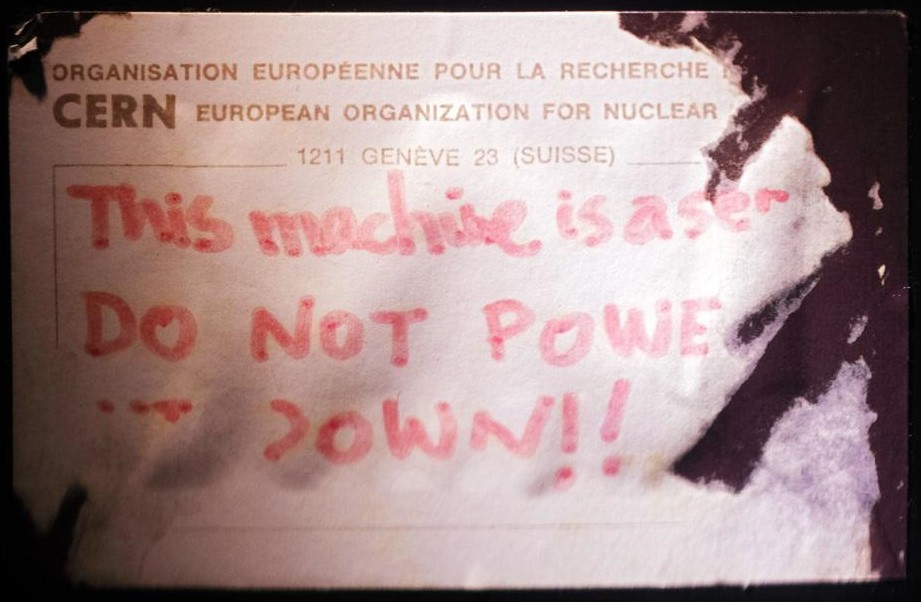
\includegraphics[scale=0.25]{./Ilustraciones/cern-server.jpg}\\
    \textbf{Fuente:} Reddint oficial del CERN [\url{https://www.reddit.com/r/CERN/}]
\end{figure}


\hfill \break
In 1991, \textit{Berners-Lee} creó una serie de tecnologías que permitían la 
conexión de documentos en un sistema hipertextual, utilizando el 
\textit{protocolo \textbf{HTTP}} y la \textit{codificación \textbf{HTML}}. 
Esto permitió a los usuarios navegar por la red y acceder a documentos 
enlazados desde cualquier parte del mundo. \\
\hfill \break
Con el tiempo, la Web se expandió y evolucionó, surgieron nuevas tecnologías como los 
motores de búsqueda, las redes sociales y las aplicaciones móviles, lo que llevó
a la denominada \textbf{Web 2.0}.\\
\hfill \break
La Web 2 se caracterizó por una mayor interactividad, el desarrollo de 
aplicaciones colaborativas y la creación de plataformas para la participación 
del usuario, como blogs, wikis y redes sociales. La Web2 también permitió la 
creación de empresas en línea y el desarrollo de nuevos modelos de negocio basados 
en la publicidad y los servicios en línea.\cite{web2Explained}\\
\hfill \break
La \textbf{Web 3}, también conocida como \textit{Web descentralizada}, 
es la siguiente evolución de la Web. La Web 3.0 se centra en la descentralización 
de la web, lo que significa que los usuarios tienen mayor control sobre sus 
datos y pueden interactuar directamente entre sí sin la necesidad de 
intermediarios centralizados.\\
\hfill \break
La tecnología clave detrás de la Web 3 es la cadena de bloques (blockchain) y 
otras tecnologías de registro distribuido (DLT), que permiten la creación de 
aplicaciones descentralizadas (dApps) y contratos inteligentes (smart contracts). 
Esto permite la creación de aplicaciones que no estén sujetas a la censura, la 
interferencia o la dependencia de un solo proveedor, lo que a su vez ofrece 
mayor privacidad y seguridad para los usuarios.\\
\hfill \break
En resumen, la Web ha evolucionado desde su creación como WWW hasta la 
actualidad de la Web3. La Web 3 representa una evolución hacia un internet 
más descentralizado y democrático, donde los usuarios tienen un mayor control 
sobre sus datos y su experiencia en línea, y donde la confianza y la seguridad 
se pueden garantizar a través de la tecnología blockchain y otros mecanismos 
de confianza descentralizados.\cite{IEEEweb3Explained}\\